\section{Aufbau der Wetterstation und deren Sensoren}
Die Wetterstation Arbon verfügt über fünf Sensoren bzw. Sensor-Einheiten: Webcam, Kombi-Wettertransmitter, Wassertemperatur-Sensoren, Pegelsensor und Sonnenstrahlungssensor. Auf der Plattform im See befindet sich lediglich ein Schaltschrank mit Datenwandlern, keine Auswerteeinheit. Sämtliche Daten werden per TCP/IP über eine Glasfaserleitung an den landseitigen Server geschickt. Abbildung \ref{img:schaltschrank} zeigt den schematischen Aufbau der Komponenten im Schaltschrank und die angeschlossenen Sensoren. Die Stromversorgung ist der Übersicht halber nicht dargestellt. Der Pegel- und Strahlungssensor wurden während der Bachelor-Arbeit ersetzt beziehungsweise hinzugefügt. In den folgenden Kapiteln werden die neuen Sensoren und deren Funktionsweise erläutert.

\begin{figure}[htbp]
	\centering
	\fbox{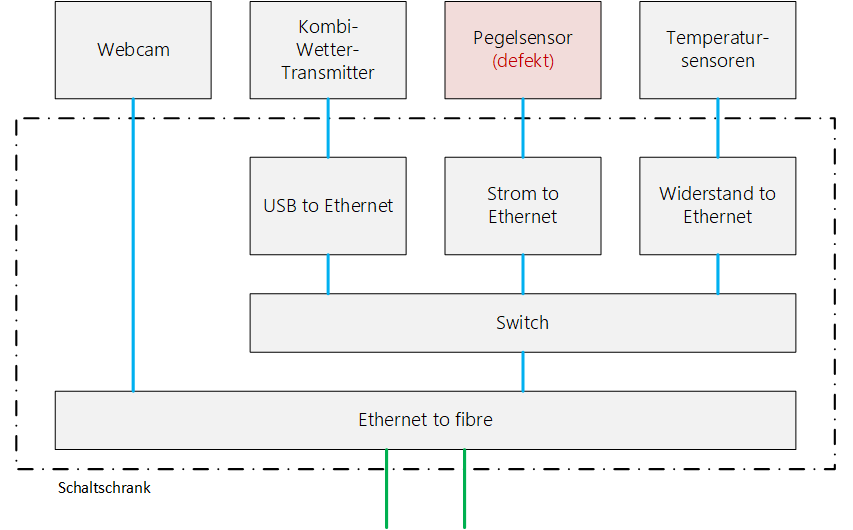
\includegraphics[width=\textwidth-2\fboxsep-2\fboxrule]{img/schaltschrank.png}}
	\caption{Hardware-Schema der Wetterstation}
	\label{img:schaltschrank}
\end{figure}




%% ############################################################################
%% Unterkapitel
%% ############################################################################
\subsection{Pegelsensor und Wellenhöhenmessung}
Die ursprüngliche Wetterstation verwendete einen hydrostatischen Drucksensor für die Messung des Wasserstands (Pegel). Der Drucksensor lieferte aber nach zehn Jahren Betrieb keine plausiblen Werte mehr, weshalb er ersetzt werden musste. Im Folgenden wird näher auf die möglichen alternativen Messprinzipien eingegangen und erklärt, wie der \emph{Pegel Konstanz} und die \emph{signifikante Wellenhöhe} definiert sind.

\subsubsection{Auswahl eines geeigneten Pegelsensors}
Für die Messung des Bodensee-Pegels wurden verschiedene Messprinzipien verglichen, mit dem Hintergedanken, die Pegelmesswerte ebenfalls zur Messung der Wellenhöhe verwenden zu können. Die Zusammenfassung der Resultate ist in der Tabelle\,\ref{tbl:pegelsensoren} aufgelistet. TOF steht für \emph{time of flight} und beschreibt ein 3D-Kamerasystem. Die Einfachheit und Robustheit des hydrostatischen Sensors überwog, sodass der alte Drucksensor durch das gleiche Produkt ersetzt wurde.

\begin{table}[htbp!]
	\caption{Gegenüberstellung der verschiedenen Pegelmess-Prinzipien}
	\label{tbl:pegelsensoren}
	\setlength\extrarowheight{4pt} % for a more "open" look
	\begin{tabularx}{\textwidth}{|>{\RaggedRight\hspace{0pt}}p{3cm}||X|X|}
	\hline
	& \bfseries Vorteile
	& \bfseries Nachteile\\

	\hline
	\textbf{Hydrostatisch}
	&
	\begin{itemize}[nosep,leftmargin=*]
	\item einfache Auswertung
	\item mechanische Dämpfung
	\item sehr kleiner Energieverbrauch
	\end{itemize}
	&
	\begin{itemize}[nosep,leftmargin=*]
	\item anfällig auf Verschmutzung
	\item keine Wellenmessung möglich
	\end{itemize}\\

	\hline
	\textbf{Ultraschall}
	&
	\begin{itemize}[nosep,leftmargin=*]
	\item berührungslos
	\item geringer Energiebedarf
	\end{itemize}
	&
	\begin{itemize}[nosep,leftmargin=*]
	\item anfällig auf Wind
	\end{itemize}\\

	\hline
	\textbf{Radar}
	&
	\begin{itemize}[nosep,leftmargin=*]
	\item windunabhängig
	\item berührungslos
	\end{itemize}
	&
	\begin{itemize}[nosep,leftmargin=*]
	\item zu geringe Auflösung für Wellenhöhe
	\item hoher Energiebedarf
	\end{itemize}\\

	\hline
	\textbf{TOF}
	&
	\begin{itemize}[nosep,leftmargin=*]
	\item Wellenhöhe messbar
	\item berührungslos
	\end{itemize}
	&
	\begin{itemize}[nosep,leftmargin=*]
	\item komplexe Auswertung
	\end{itemize}\\

	\hline
	\textbf{Boje}
	&
	\begin{itemize}[nosep,leftmargin=*]
	\item Wellenhöhe messbar
	\end{itemize}
	&
	\begin{itemize}[nosep,leftmargin=*]
	\item wartungsintensiv
	\item Batteriebetrieb
	\end{itemize}\\

	\hline
	\end{tabularx}
\end{table}

\subsubsection{Definition des Pegel Konstanz}
Die Uferlinie des Bodensees wurde 1990 von der IGKB\footnote{IGKB: Internationalen Gewässerschutzkommission für den Bodensee} bei Mittelwasserstand festgelegt. Der Pegelstand in Konstanz ist ein Relativmaß. Er bezieht sich auf den Pegelnullpunkt, der in Konstanz bei 391,89m ü NN liegt. Der Pegel Romanshorn gibt die geodätische Höhe des Wasserstandes in Meter über Meer wieder~\cite{igkbPegel}. Der Zusammenhang der verschiedenen Pegelgrössen ist in Abbildung\,\ref{img:pegelKonstanz} dargestellt. Links oben (violett) befindet sich die Skala für den Pegel Konstanz. Die offizielle Hochwassermarke liegt bei einem Pegel von 4,80 Metern.

\begin{figure}[htbp!]
	\centering
	\fbox{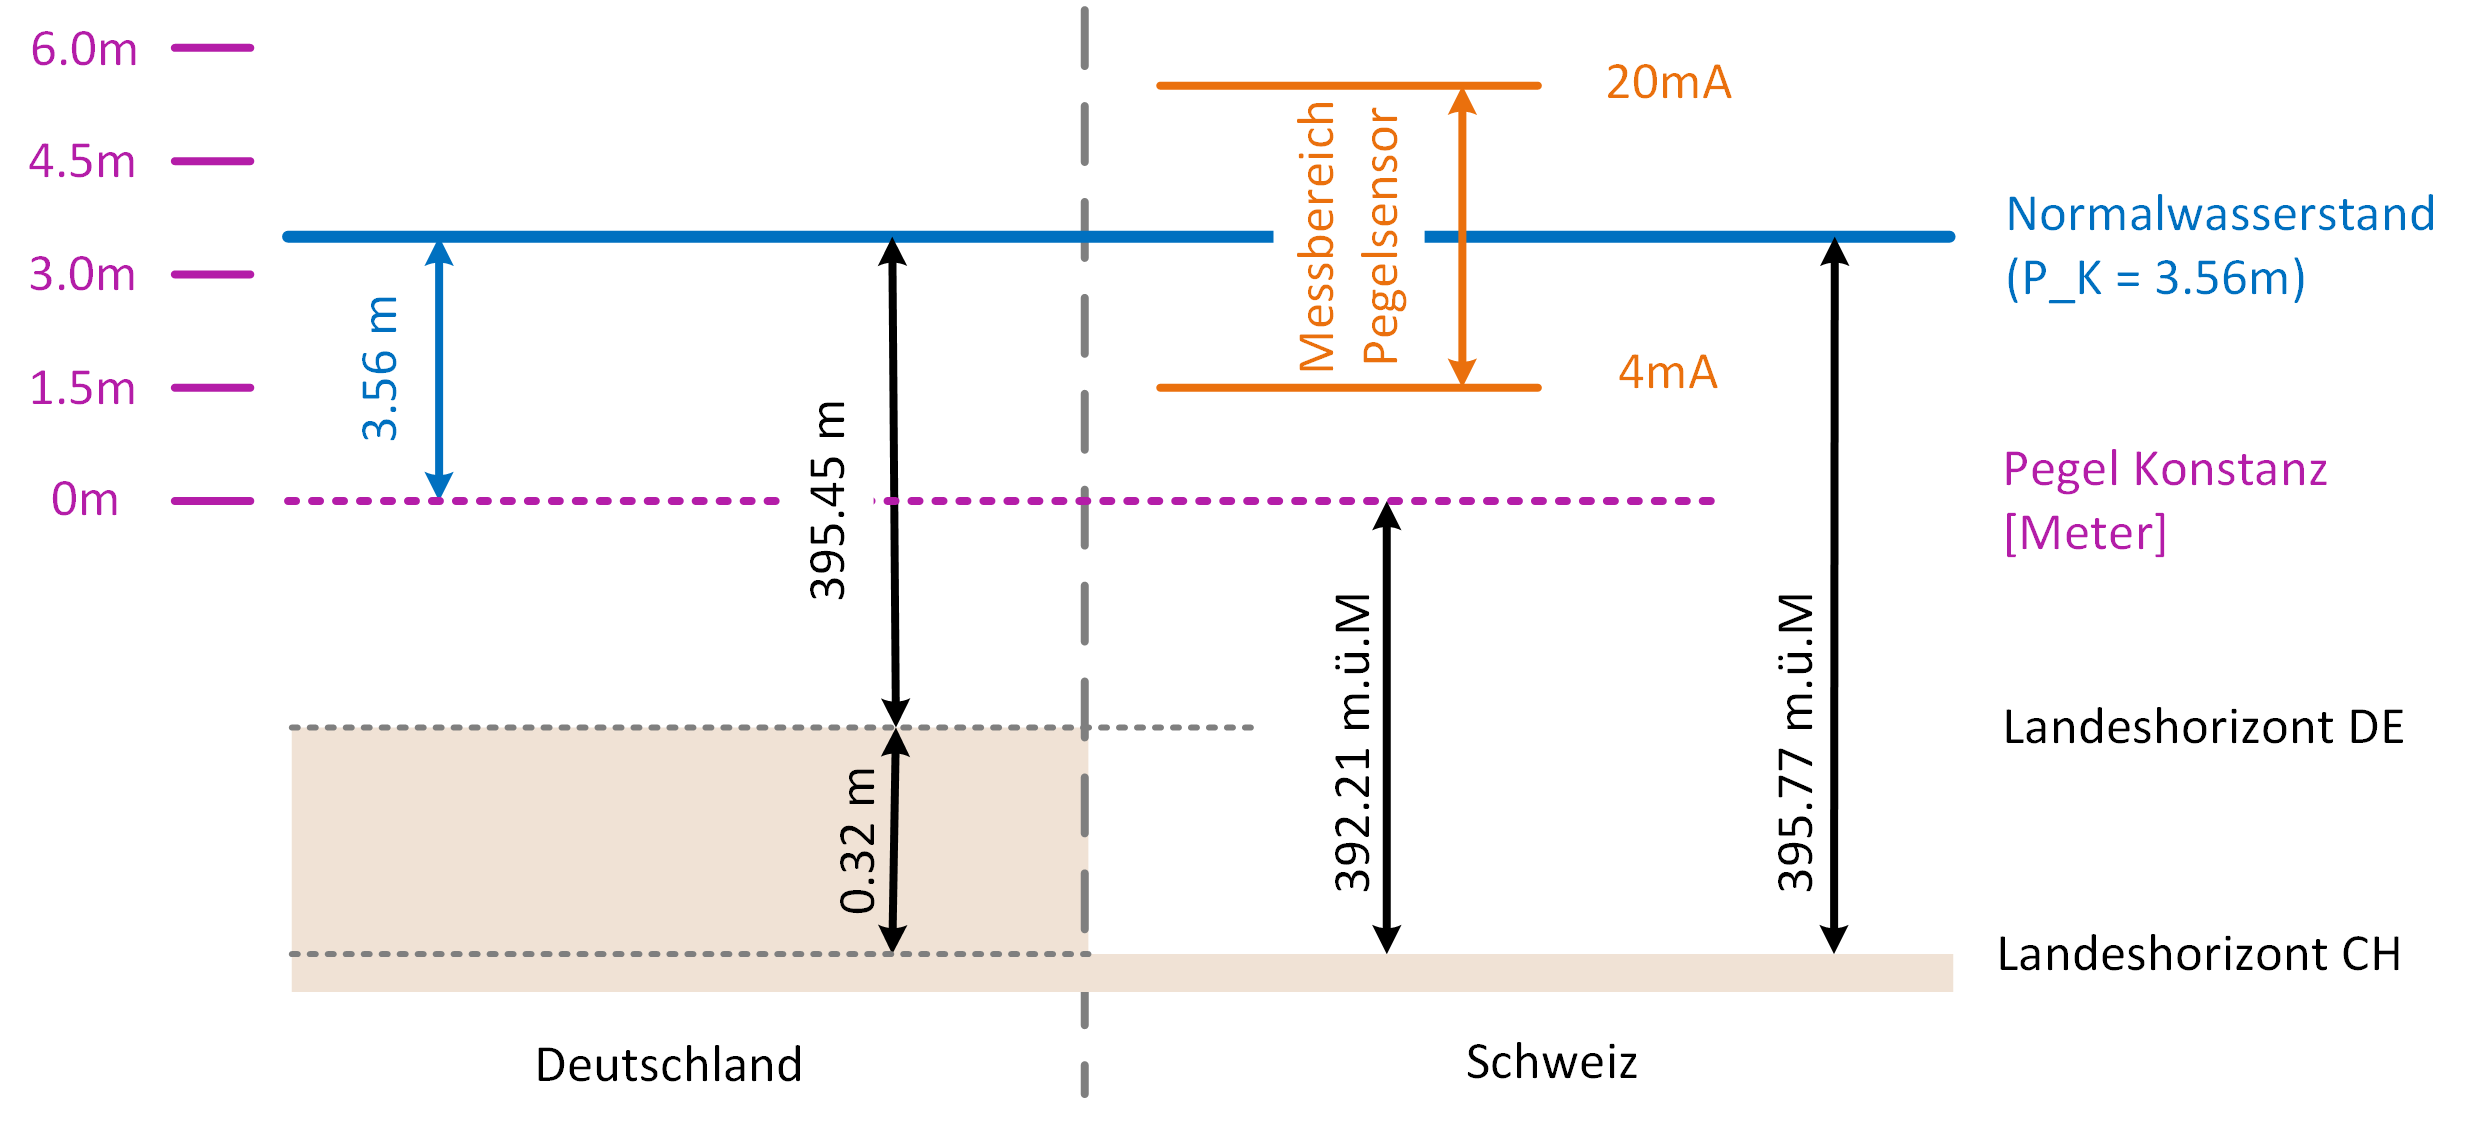
\includegraphics[width=\textwidth-2\fboxsep-2\fboxrule]{img/pegelKonstanz}}
	\caption{Berechnung des Pegel Konstanz und Messbereich des Sensors}
	\label{img:pegelKonstanz}
\end{figure}

\noindent
Der Pegelsensor liefert einen Strom von 4...20\,mA bei einer Messhöhe von 4\,Metern. Der Pegelsensor ist 1.75\,Meter über dem Pegelnullstand angebracht.
Die Berechnung des Pegel Konstanz aus dem Messwert erfolgt demnach gemäss der Formel \ref{eq:Pegelformel}. Aus technischen Gründen ist 1.75\,m bzw. 5.75\,m der tiefste bzw. höchste von der Wetterstation messbare Pegel, wie in Formel\,\ref{eq:Pegelmin} und \ref{eq:Pegelmax} berechnet.

\begin{equation}
\label{eq:Pegelformel}
P_{K} = m*x + q = 4/16 * x + 0.75
\end{equation}

\begin{equation}
\label{eq:Pegelmin}
P_{g,u}= P_{K}(x=4)= 4*0.25 + 0.75 = 1.75
\end{equation}

\begin{equation}
\label{eq:Pegelmax}
P_{g,o} = P_{K}(x=20)= 20*0.25 + 0.75 = 5.75
\end{equation}

wobei:
\begin{conditions}
P_{K}    &  Pegel Konstanz [m]\\
P_{g,u}   &  Tiefster messbarer Pegel [m]\\
P_{g,o}   &  Höchster messbarer Pegel [m]\\
x        &  Messwert [mA]\\
m        &  Auflösung des Sensors [m/mA] (0...4m bei 4...20mA)\\
q        &  Offset [m] \\
\end{conditions}

\noindent
Der Pegelsensor ist an einem Web-Interface angeschlossen, welches den Strom-Messwert über eine Web-Schnittstelle zur Verfügung stellt. Der aktuelle Messwert kann so bequem mittels \emph{GET}-Abfrage aufgerufen werden, wie in Listing\,\ref{lst:curlPegel} aufgezeigt. Da das Web-Interface nur schwach (Passwortabfrage in Klartext) gegen unerwünschte Zugriffe geschützt ist, wurde die Firewall der Wetterstation so konfiguriert, dass nur vom Hosting-Server aus die Abfrage durchgeführt werden kann (IP-Einschränkung).

\vspace{3mm}
\begin{lstlisting}[label=lst:curlPegel,caption=Abfrage des Pegelsensor-Wertes über das Hostpoint-Terminal, language=Python, style=htmlcssjs]
[igwetter:] $ curl http://webcam.wetter-arbon.ch:50506/single1
11,748 mA
\end{lstlisting}
\vspace{3mm}

\subsubsection{Definition der signifikaten Wellenhöhe}
Ursprünglich war geplant, mit dem Pegelsensor ebenfalls die Wellenhöhe zu messen. Dies ist aber mit dem gewählten Pegelsensor bzw. dessen Montage nicht möglich. Das Einbaurohr wirkt als Tiefpass-Filter und verunmöglicht die Messung von schnellen Wassersäuleänderungen. Nichtsdestotrotz und im Hinblick auf eine allfällige Erweiterung der Wetterstation um einen Wellenhöhensensor soll hier kurz die Definition der signifikanten Wellenhöhe erläutert werden.

Als Seegang bezeichnet man die winderzeugten Oberflächenwellen des Meeres. Da sich der Seegang in der Natur als eine Überlagerung vieler Einzelwellen darstellt, werden zu dessen Beschreibung statistische Größen wie z.B. die signifikante Wellenhöhe verwendet. Die Definition einer signifikanten Wellenhöhe geht auf die visuelle Bestimmung einer charakteristischen, den Seegang beschreibenden Wellenhöhe zurück. Die signifikante Wellenhöhe wird gemäss der \emph{List of sea state parameters}~\cite{1986Iahr} definiert als die mittlere Wellenhöhe der 33\% höchsten Wellen in einem repräsentativen Zeitraum (z.B. 20\,Minuten).

%% ############################################################################
%% Unterkapitel
%% ############################################################################
\subsection{Wassertemperatur-Sensoren}
Die Wetterstation verfügt über acht Wasser-Temperatursensoren (PT100-Elemente), die im Abstand von 0.5\,m in einem Rohr angebracht sind. Die offizielle Wassertemperatur wird einen Meter unter der Wasseroberfläche gemessen. Für Schwimmer ist aber die Temperatur auf einem halben Meter unter der Wasseroberfläche interessanter, weshalb dieser Wert ebenfalls ausgelesen und gespeichert wird. Das Schwimmbad Arbon bezieht bereits heute für seine Webseite\footnote{ \url{https://www.schwimmbad-arbon.ch}} die Wassertemperatur von der Wetterstation.
% \Diskussionspunkt{- Wo ist Wassertemperatur definiert? }

\begin{figure}[htbp]
	\centering
	\fbox{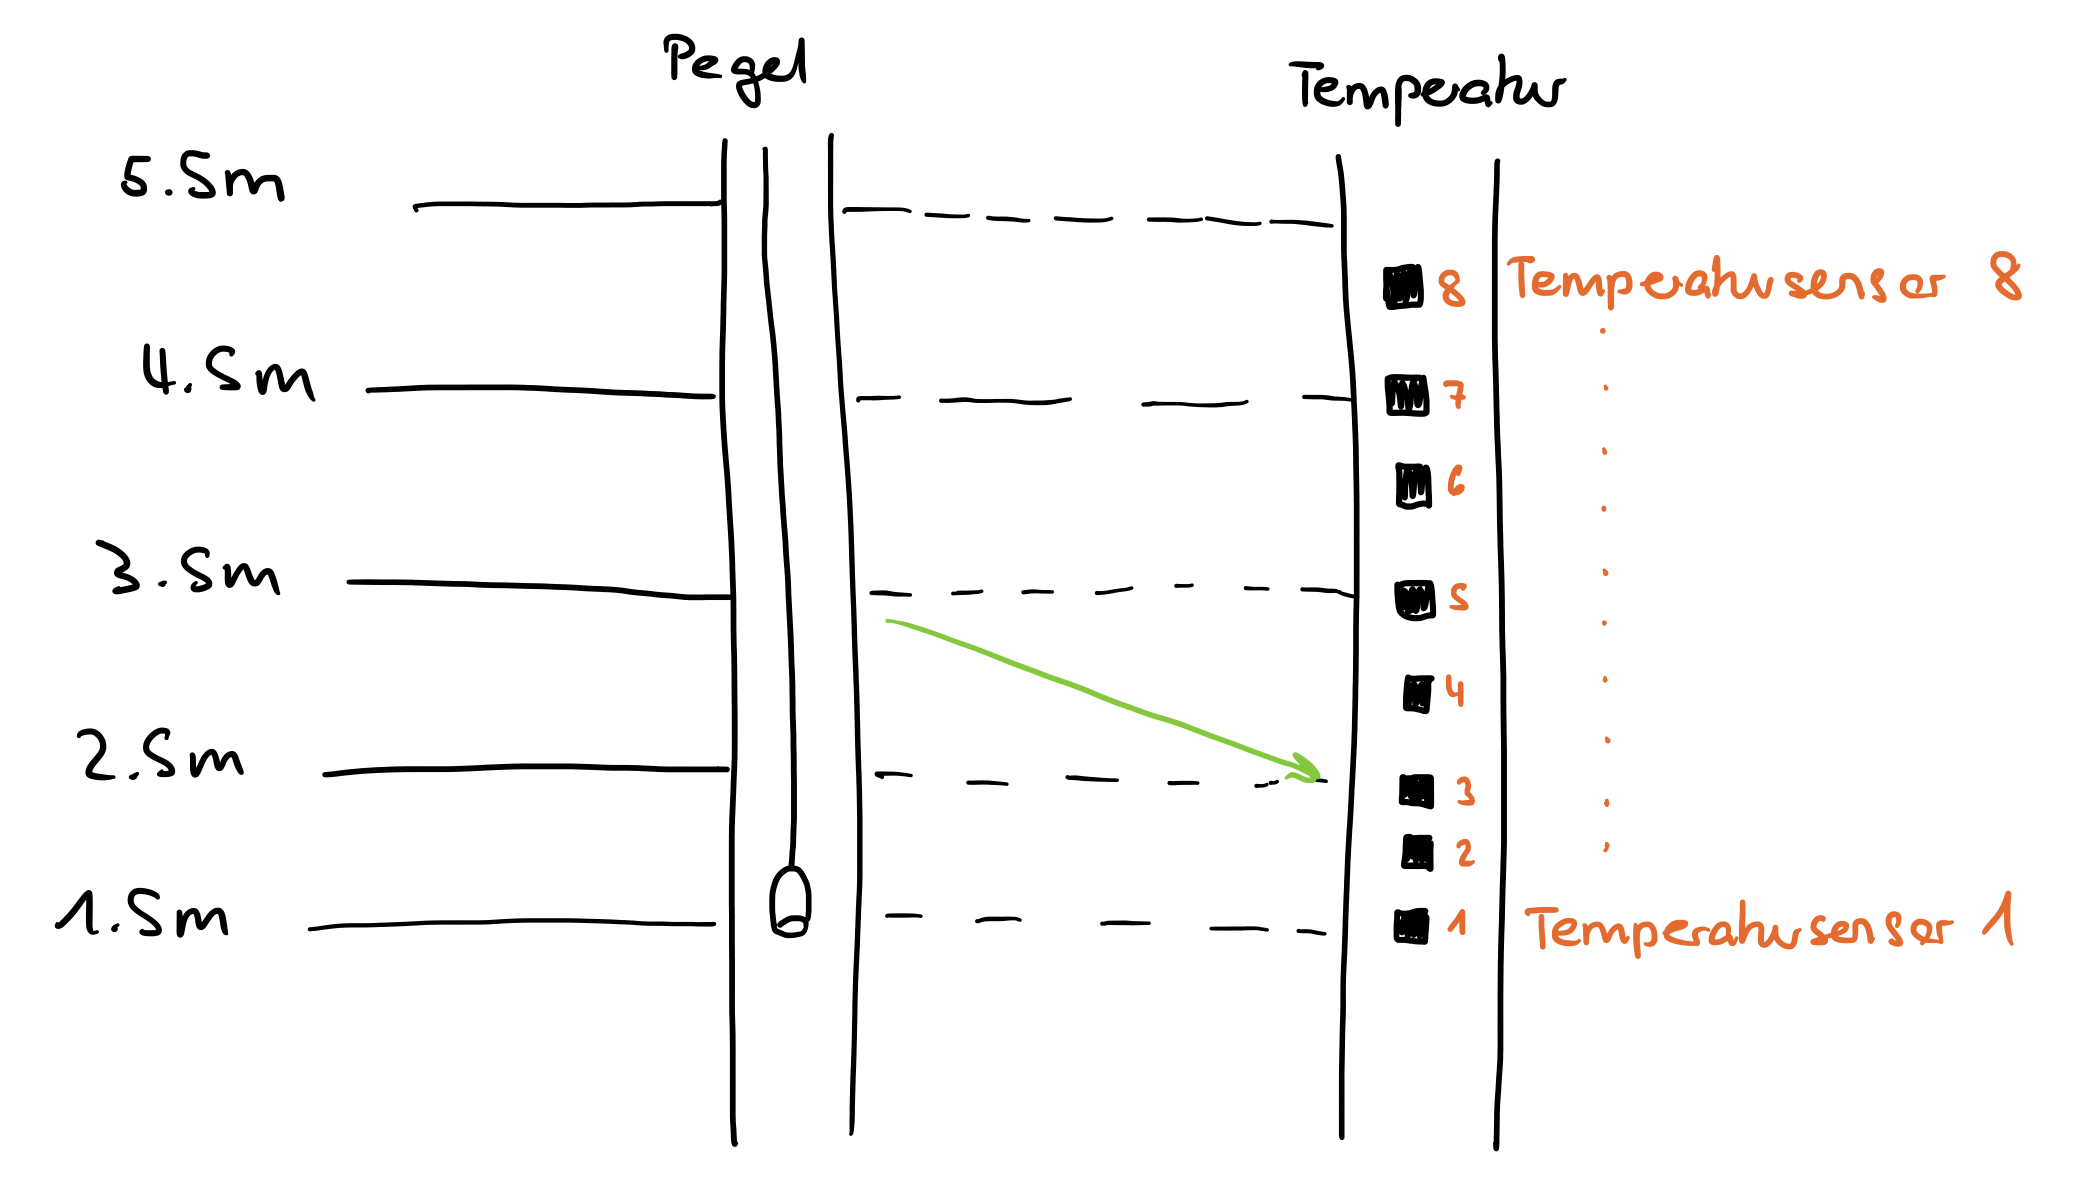
\includegraphics[width=\textwidth-2\fboxsep-2\fboxrule]{img/wassertempsensoren}}
	\caption{Zusammenhang zwischen Pegel und PT100-Temperaturwiderständen}
	\label{img:wassertempsensoren}
\end{figure}

\subsubsection{Auswahl des richtigen Temperatursensors anhand des Pegels}
Damit der richtige Temperatursensor ausgewählt werden kann, muss der Pegel bekannt sein. Abbildung \ref{img:wassertempsensoren} zeigt das Prinzip schematisch auf. Mittels Cronjob werden sämtliche Temperatursensoren ausgelesen und in einem Array gespeichert. Anschliessend wird mit Hilfe des Pegelwerts der korrekte Wert entnommen, wie in Listing \ref{lst:tempSelect} beispielhaft aufgezeigt.

\begin{lstlisting}[label=lst:tempSelect,caption=Auswahl des richtigen Temperatursensors, language=Python, style=py]
if waterlevel >= 3.5 and waterlevel <= 4.0:
    watertemperature100cm  = float(temperatureArray[3])
    watertemperature50cm   = float(temperatureArray[4])
\end{lstlisting}




\subsubsection{Annäherung des defekten PT100-Widerstands}
Die Temperatursensoren waren mehrere Jahre nicht in Betrieb. Zur Kontrolle wurden deshalb während sechs Wochen alle Temperaturdaten aufgezeichnet. Ein Auszug der Messdaten ist in Abbildung \ref{img:tempSensoren} dargestellt. Es lässt sich erkennen, dass sich die Sensoren\,1 bis 4 im Wasser, und die Sensoren\,6 bis 8 über Wasser befinden. Beim Sensor\,5 ist nicht klar, ob er im oder über dem Wasser ist. Auf Grund der Messdaten lässt sich auch kein konstanter Offset gegenüber den benachbarten Sensoren ermitteln.

\begin{figure}[htb!]
	\centering
	\fbox{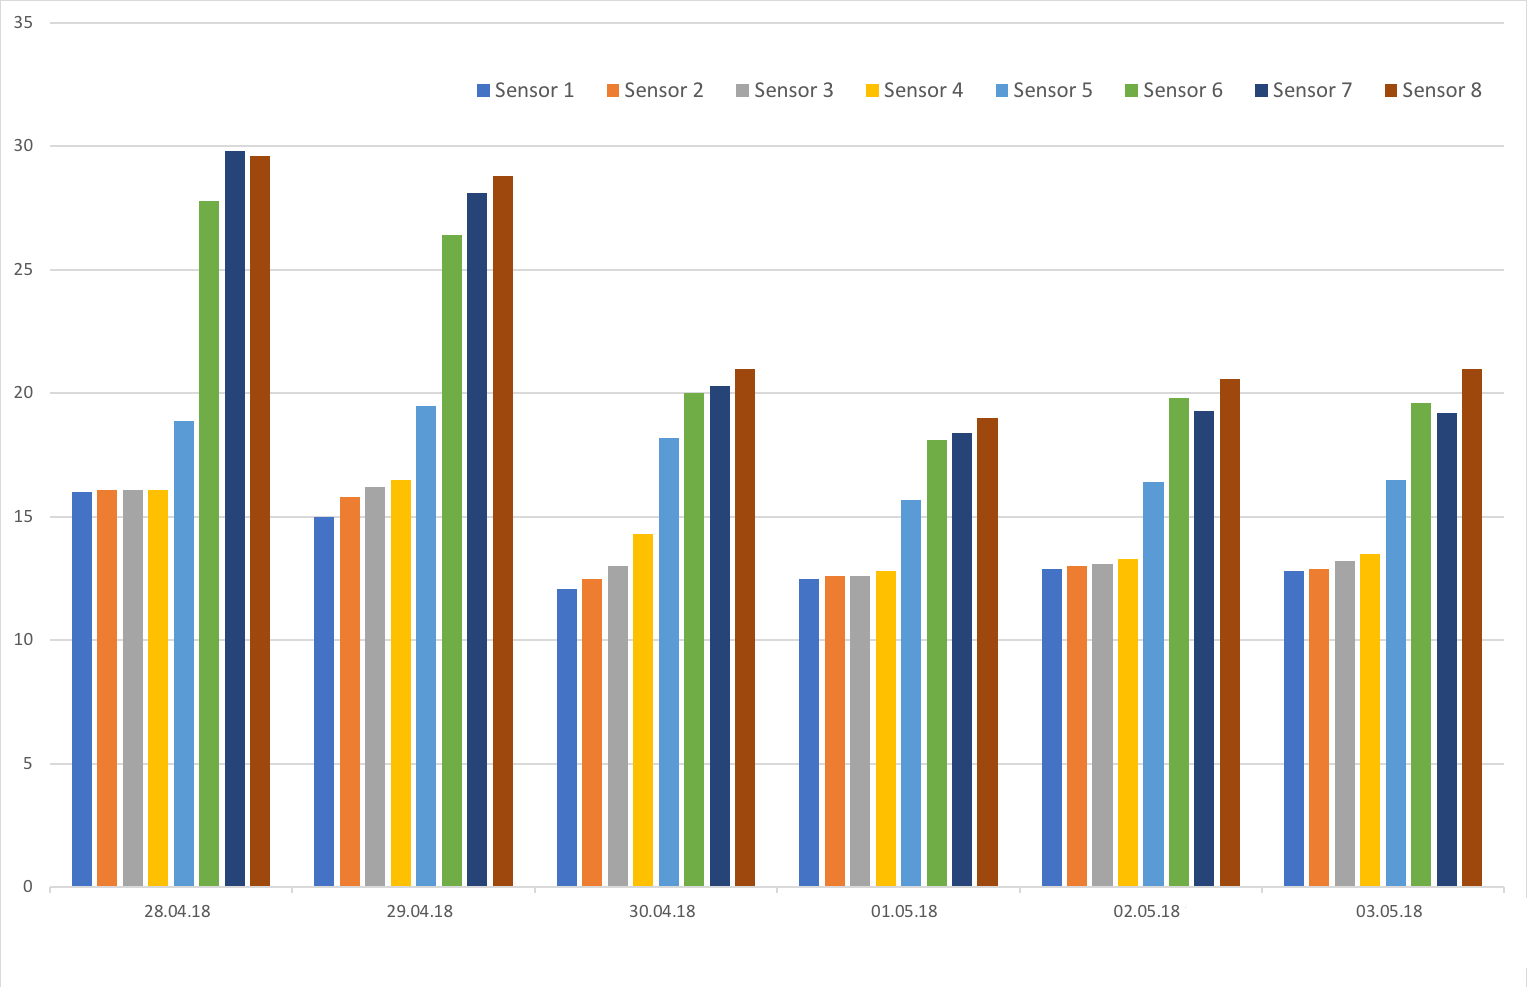
\includegraphics[width=\textwidth-2\fboxsep-2\fboxrule]{img/tempSensoren}}
	\caption{Messreihe aller Temperatursensoren}
	\label{img:tempSensoren}
\end{figure}

\noindent
Der fehlende bzw. falsche Wert wurde trotzdem durch einen Offset angenähert. Ein Offset von drei Grad hat sich als meistens korrekt erwiesen. Der Offset wird direkt beim Auslesen der Temperaturdaten abgezogen, wie in Listing \ref{lst:tempOffset} aufgezeigt.

\vspace{3mm}
\begin{lstlisting}[label=lst:tempOffset,caption=Offset des defekten Temperatursensors, language=Python, style=py]
offset = -3  # [Grad]
temperatureArray[4] = float(temperatureArray[4]) + offset
\end{lstlisting}


%% ############################################################################
%% Unterkapitel
%% ############################################################################
\subsection{Sonnenstrahlungssensor}
Die Sonnenscheindauer dient der näherungsweisen Bestimmung der Sonneneinstrahlung an einem bestimmten Ort und gibt gleichzeitig Hinweise auf Zeit und Stärke der Bewölkung. Sie diente ursprünglich der Charakterisierung von Kurorten. Dabei wurde die psychologische Wirkung von Sonnenlicht auf das menschliche Wohlbefinden hervorgehoben. Auch heute noch werden die Sonnenstunden verwendet, um touristische Ziele zu fördern.

\noindent
Zur Messung der Sonnenstunden gibt es gemäss \emph{Guide to Meteorological Instruments and Methods of Observation (WMO)}~\cite{WMO2014Gtmi} fünf Messprinzipien, wobei die pyranometrische Methode die einfachste und kostengünstigste Methode darstellt. Dabei misst ein Pyranometer die Globalstrahlung\,$G$, welche anschliessend zur Abschätzung der Sonnenscheindauer verwendet wird. Das Messprinzip des Pyranometers und die Berechnung der Sonnenstunden werden im Folgenden erklärt.

\subsubsection{Funktionsprinzip eines Pyranometers}
Das Pyranometer basiert auf dem Messprinzip eines Thermoelements. Die einfallende Strahlung trifft auf einen Absorber, welcher erwärmt wird. Die Wärme fliesst dann über das Gehäuse an die Umgebung ab (siehe Abbildung\,\ref{img:pyranometer}. Die Strahlungsleistung ist dabei proportional zum Wärmestrom beziehungsweise zur Temperaturdifferenz vom Absorber zum Gehäuse. Die Temperaturdifferenz wird mit Thermoelementen gemessen. Um die Signalspannung zu erhöhen, werden mehrere Thermoelemente in Reihe zu einer Thermosäule geschaltet. Durch das thermische Messprinzip ist ein Pyranometer träge. Die Verzögerung liegt bei wenigen Sekunden.

\begin{figure}[htbp]
	\centering
	\fbox{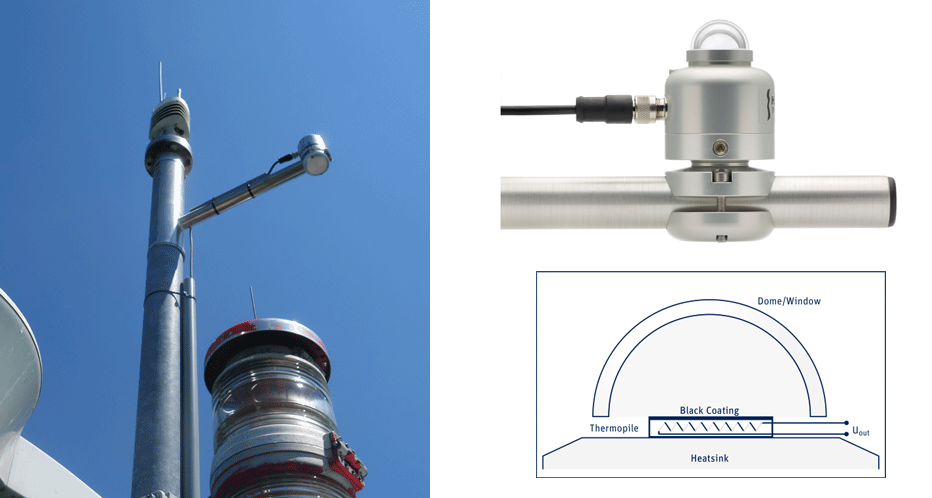
\includegraphics[width=\textwidth-2\fboxsep-2\fboxrule]{img/pyranometer.png}}
	\caption{Montageort und \href{http://www.kippzonen.com/News/572/The-Working-Principle-of-a-Thermopile-Pyranometer}{Funktionsprinzip} eine Pyranometers }
	\label{img:pyranometer}
\end{figure}


\subsubsection{Berechnung der Sonnenscheindauer}
Die Sonnenscheindauer (SD) kann aus den minütlichen Messwerten der Globalstrahlung\,$G$ berechnet werden~\cite{WMO2014Gtmi}. Dazu muss zuerst der Schwellwert\,$G_{thr}$, wie in der Formel\,\ref{eq:Sonnenstunden} dargestellt, berechnet werden. Der Schwellwert ist das Produkt aus mehreren Parametern, welche vom Standort und der Sonnenposition abhängig sind. Der Zähler für die Sonnenstunden wird um eine Minute erhöht, wenn der Messwert grösser ist als der Schwellwert und der Sonnenwinkel mindestens 3 Grad beträgt.

\vspace{3mm}
\begin{equation}
\label{eq:Sonnenstunden}
G_{thr} = A + B \cdot cos \left(\frac{360\cdot d}{24\cdot 365}\right) \cdot 1080 \cdot sin(h)^{1.25}
\end{equation}
\vspace{3mm}

wobei:
\begin{conditions}
G_{thr}  &  Schwellwert der Globalstrahlung \\
d        &  Laufende Stunde seit Anfang Jahr \\
h        &  Elevationswinkel der Sonne in Grad \\
A        &  empirisch bestimmter Koeffizient (0.65) \\
B        &  empirisch bestimmter Koeffizient (Saisonalität) (0.15) \\
\end{conditions}

\noindent
Zur Bestimmung der beiden Koeffizienten $A$ und $B$ konnte auf die Messwerte des NTB in Buchs zurückgegriffen werden. Da die Strahlungsintensität von Buchs und Arbon vergleichbar sind (gleiche geografische Breite und Höhe), wurden die Koeffizienten direkt übernommen. Abbildung\,\ref{img:radiation} zeigt die Darstellung von Sonnenscheindauer und Strahlung, sowie deren Verlauf über die letzten beiden Tage, wie sie auf der Webseite angezeigt werden.

\begin{figure}[htbp]
	\centering
	\fbox{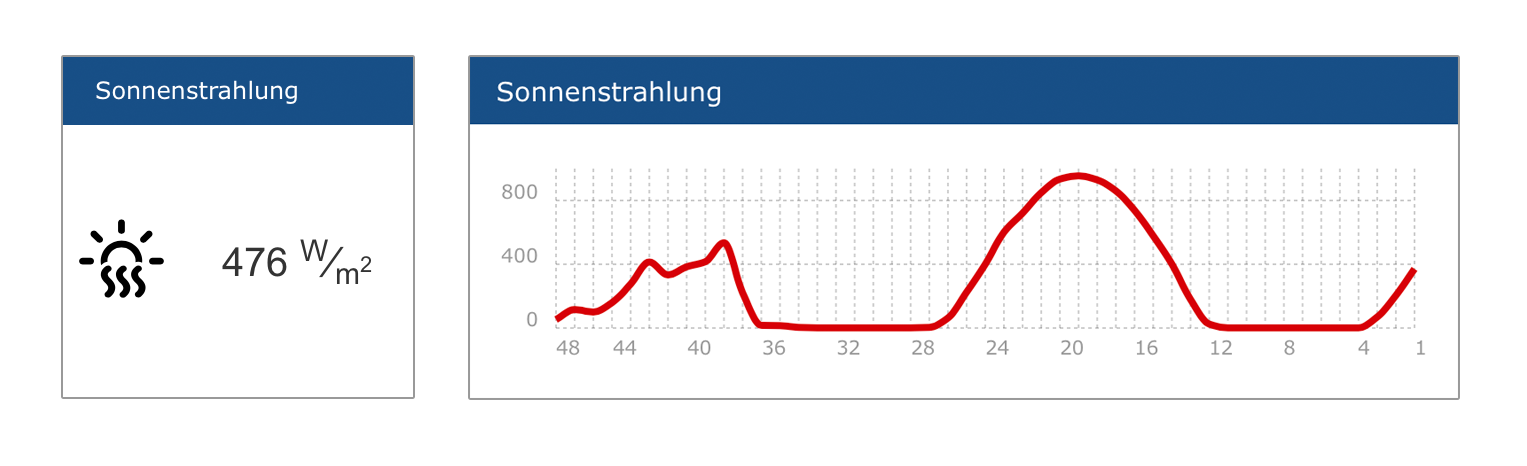
\includegraphics[width=\textwidth-2\fboxsep-2\fboxrule]{img/radiation}}
	\caption{Darstellung des aktuellen Messwerts und des Strahlungsverlaufs}
	\label{img:radiation}
\end{figure}

\subsubsection{Verwendung für PV-Anlagen}
Das webbasierte Tool PVGIS\footnote{\url{http://re.jrc.ec.europa.eu/pvgis/apps4/pvest.php}}, welches durch das europäische \emph{Joint Research Centre} (JRC) entwickelt wurde, ist ein beliebtes Tool, wenn es darum geht, den Ertrag einer PV-Anlage vorherzusagen. Die Daten basieren auf der Interpolationen von Messungen von diversen Boden-Messstationen. Es liegt nahe, diese Berechnung mit unseren Messwerten zu vergleichen. PVGIS berechnet für den Standort Arbon im Monat Juli Strahlungswerte von bis zu $900 \nicefrac{W}{m_2}$, gemäss Abbildung\,\ref{img:pvgis}.

\begin{figure}[htb!]
	\centering
	\fbox{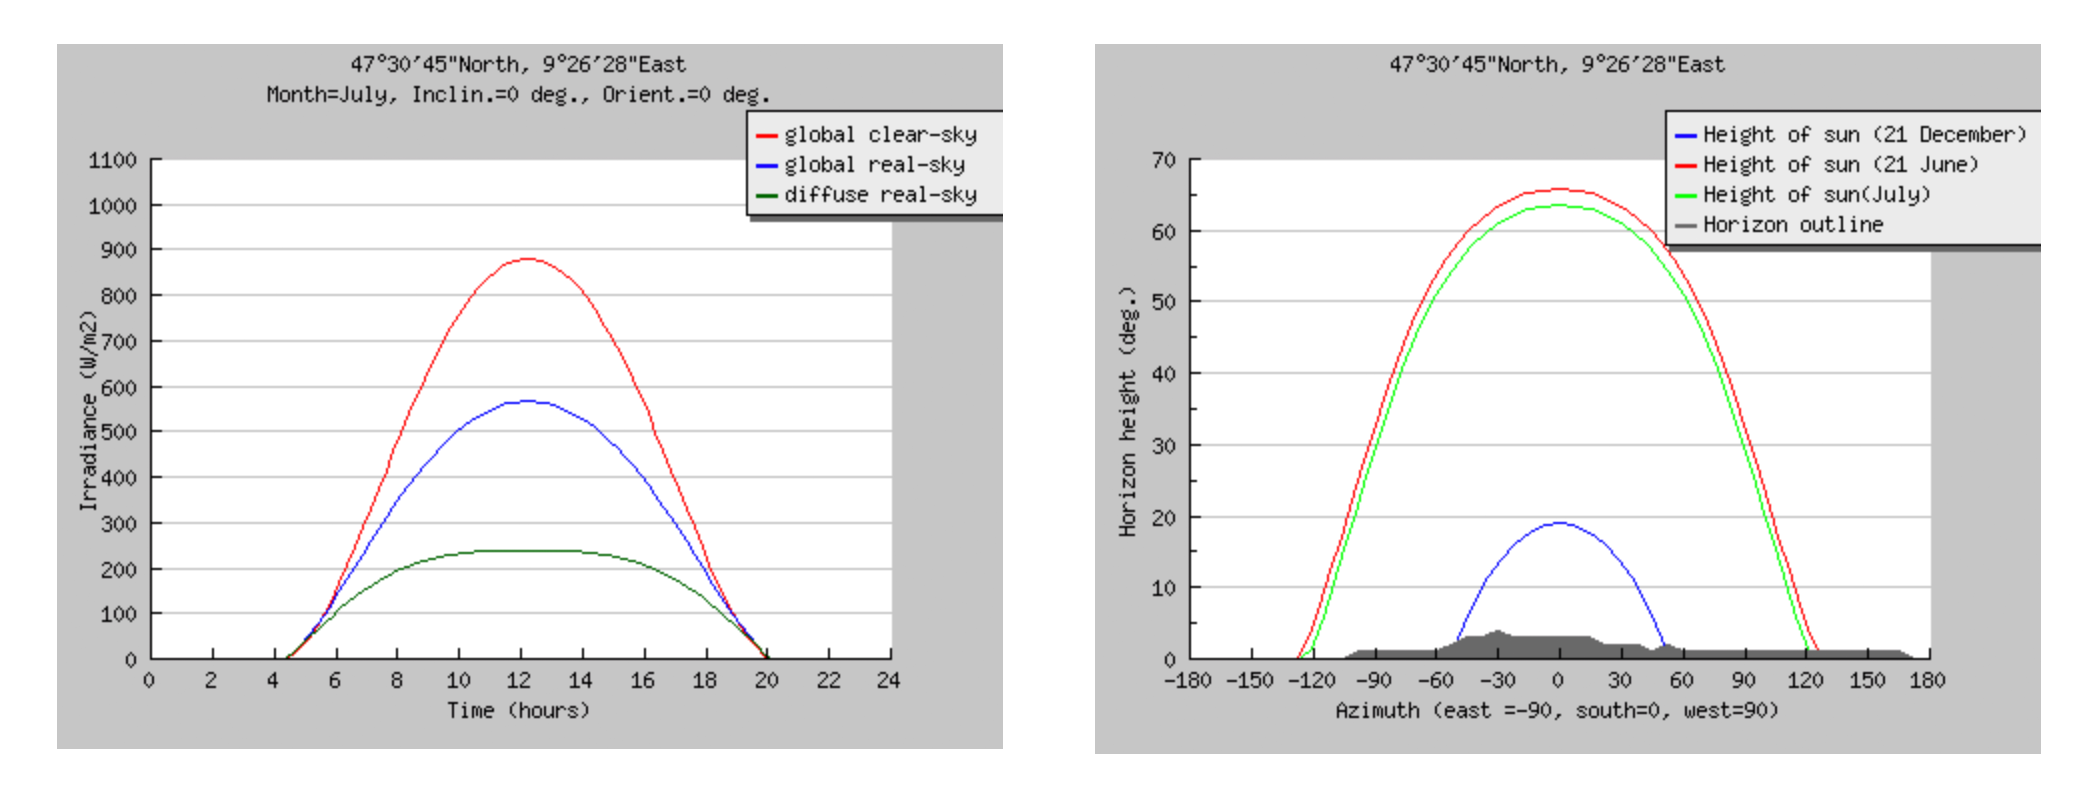
\includegraphics[width=\textwidth-2\fboxsep-2\fboxrule]{img/pvgis}}
	\caption{Interpolierte Strahlungsvorhersage und Sonnenwinkel für Arbon}
	\label{img:pvgis}
\end{figure}
